\chapter{Introduction}
The main target of this paper is to uncover what effects do different software implementations in virtual reality applications have on percieved user immersion. This research will be achieved through the development of a series of virtual reality test applications that will explore factors such as the implementation of sound design, hands on interaction, level design and movement.
These factors

\section{Background}
h
\section{The Question}
The question is what effects do different software implementations in vritual reality applications have on percieved user immersion. 



This project has been taken up to fill out the requirements for a Bsc. In computing (information technology) at Technical University Dublin Blanchardstown in Dublin, Ireland. The objective of this project is to research and develop virtual reality environments which are widely accessible and immersive. The research data may be used by future developers to create immersive experiences.  
Due to the technologies in this paper are relatively new, the abundance of present research is sparse in comparison to other topics of research. 

Although sparse and the this type of project not being openly recommended by the project supervisors, the writers of this paper have a personal interest in the topic and would like to aid the progress of this technology.  Therefore, some of the goals of this paper are to show the tools, data and test methods used in this project to create an accessible and immersive virtual reality environment. 

%-------------------------------AIMS AND OBJECTIVES-------------%

\chapter{Aims and Objectives of this Project}

\subsection{Immersion in virtual reality environments }
One of the projects main goals is to create several immersive virtual reality environments. To do that there was prior research conducted as stated in the literature review. To create an immersive virtual reality environment there must be a lot of interactivities available to the user. Firstly, there should be a tutorial which should introduce users to the core mechanics of using a virtual reality headset and controller. Whether this just be picking up a glass or even picking up and turning on and off a flashlight, this makes it so users are more familiar in the environment that will be presented for them to test. 

Another way to make this project immersive is to make all assets in the environment the proportional to how they are in real life as if the assets are too small this could distract from properly testing and could affect results. Tests will then be needed for each interactive object in the environment to make sure that this doesn’t happen. 

Immersion will be talked about in the literature review section of this paper and expands on points made in this  

\subsection{Accessibility in virtual reality}
Accessibility in virtual reality is very important, this is because many users may have some form of disability or just get motion sick easily. There are many ways to create a safe and accessible virtual reality environment. Whether it be through making the art style in the environments have a low polygon count as this may reduce users feeling motion sick and helps make sure the environment can run at a high frames per second. Having modes where the user can just teleport to section can also help motion sickness users as this stops the feelings of moving. This project could also have a feature where the user can turn off the smooth turn feature and make it so they can turn at varying degrees with ninety degrees being the largest amount a user can snap to while turning. 

To help users with disabilities there can be several settings enabled. Letting users have a sit-down mode helps let users who are wheelchair bound or have issues standing overall have access to the virtual reality environments. There is more information in the accessibility section of the literature review that shows several more ways this project can become more accessible to more users. 

\subsection{Making the project testable}
To make the project testable there will have to be several measures in place, these are: 

Making sure that there is a feedback section at the end of each experience laid out for the user and have it ask questions such as, did you find this experience enjoyable, immersive, and accessible to everyone. Another important section to add in might be another section in which the user can provided their own feedback and how the project could be improved. 

Another way this project will be testable is through a heart rate monitor. To make this work the user will have to put on a heart rate monitor and play through several experiences available in this project testing environment. To monitor the results there will have to be a person gathering data for each experience, it would be a clever idea to test the highest and lowest heart rate. This could help show which type of experiences either scare the user, give the user an adrenaline rush or keep the user relaxed. 

\subsection{Risk analysis}
This project may have many obstacles that do come up. To circumvent these issues, they must made be made known before starting the project. While it is not a guarantee this issue will occur, it is better if they are known so that they do not temporarily or completely stop all progress on the project. 

An issue that may occur while making the project is finding people to do the tests on, there is several reasons why a person may not want to test the project. A large reason currently as of writing this document is COVID-19. Many people may not feel safe sharing a virtual reality headset which has been worn by multiple people, to try and help make sure people do feel safer while testing the project hand sanitiser should be available so users can safely pick up the controllers and the headset should also be sanitised to make sure the user is as safe as possible while conducting the test. It is also best to test people randomly as testing on people who are close to the people conducting the experiment may create a bias discrediting the feedback section results.  

Another issue could be time constraints and finding the time to run these tests. Throughout the year there could be other modules that require a lot of attention, this could lead to delays with the plan set out with the Gantt chart or make a lot of challenges that will occur during the year a lot more stressful to deal with. 

Hardware limitations may also play a large part in the getting this project complete. This could be due to limitation of the computer and virtual reality headset running the virtual reality environments. 


%-------------------------------LITERATURE REVIEW-------------%
\chapter{Literature Review}

\section{Immersion}
Immersion is defined as being present or involved in an activity or experience, to the point of where one feels like they are truly part of it.  

\subsection{Immersion VIA Interaction}
In a paper that was written by (Slater et al., 2009), presents interaction and reaction as core component of creating an immersive experience. Their interpretation of immersion is that it is a state of reaction to the simulated data which the virtual environment is made up of. Introducing the capability to interact with this sensory data allows the user to play a more physical role in this space. Rather than a passive interaction when the user is presented with an entity, they are able to interact with said item using their own hands. In the paper they establish that a realistic interpretation of reality is not detrimental to introduce the factor of immersion. “High presence does not demand high fidelity to physical reality, but rather that people do respond, and be able to respond, as if the sensory data were physically real. This approach makes “presence” directly observable and measurable –both with respect to observations of others, and with respect to knowledge of one’s own behaviour–.” (Slater et al., 2009) 3.1.1 Method of interaction Expanding further on the topic of interaction, users might be presented with various forms of entities such as doors, buttons, hand-held objects, or even virtual representations of living organisms such as animals or people. In a paper by Doug A. Bowman and Larry F. Hodges titled ‘An evaluation of techniques for grabbing and manipulating remote objects in immersive virtual environments’ it is discussed that there are various 6 Abbreviations 7 methods of remotely interacting with objects in a virtual space. They make the point that “Instead of issuing an abstract command or specifying coordinates and rotation angles, users may reach out a hand, grab an object (using a button or a gesture), and move it around the virtual environment (VE) using natural, physical motions”. Although interacting with objects remotely is not the goal of the project it remains that the focus is on allowing the user to use their own hands to interact with objects in a natural manor using an interface such as the controllers mentioned above.  

\subsection{Immersion VIA Sound}
It is true that a focus on interaction and visuals is important for immersion however the topic of sound design cannot be left out. The creation of immersive soundscapes can be used to further increase the feel of immersion through the introduction of ambient sounds and the simulation of surround sound. In a book written by Roginska and Geluso titled ‘Immersive Sound: The Art and Science of Binaural and Multi-Channel Audio’ they discuss virtual auditory spaces which use an array of auditory techniques to generate immersion. “A virtual auditory space is an acoustic environment created through the use of loudspeakers or headphones designed to replace or augment the natural listening environment” (Roginska and Geluso, 2017). They make a point of how sound can be used to ground the end user to a specific point even if the visual environment is in flux. Such a method can be used in virtual reality to help battle the potential motion sickness issues which has been a commonly occurring problem with HMD’s.  

\subsection{Immersion VIA Perspective}
Due to the first-person perspective that is utilized in virtual reality it is important to depict the virtual space with context of the user. For example, If the height of the perspective differs from the height of the user it might be jarring and potentially cause motion sickness. Most modern HMDs are capable of measuring the height of the user by requesting them to calibrate the device in the initial setup. This calibration is typically done through asking the user to place the controllers on floor level to determine the base and then the user must stand up which allows the device to calculate the distance between the floor and eye level. Another concept to consider in virtual reality perspective is depth. Creating the illusion of depth is generally done through perspective projection, which is a common technique used in 3D rendering. However, the previously mentioned stereoscopic technology used in HMD’s allows for the brain to evaluate depth in a more natural manner. 

\section{Accessibility}
While Virtual reality has been popularised by video games, Virtual reality has been developed to be used in many things other than gaming over the years. One of these is helping older people receive effective physical activity to improve their health. It is important to the group to make the video game as accessible as possible for people who may be limited in their movement and make sure they can use the video game as anyone else would. 

To do this research on how people of age used virtual reality games and systems for their own benefit. One of the studies shown looked at showed that older people who used a virtual reality headset daily for over ten weeks had "reduced fatigue on the Fatigue Severity Scale, weight and waist circumference in a case series of individuals with systemic lupus erythematosus" (Miller et al., 2014) it also states that virtual reality also helped with people who suffered with Parkinson's disease.

In these set of studies, it was shown that playing a virtual reality video game or experience can also enhance well-being by allowing the people participating in the study to play video games together, this helped them to get "improvements in loneliness(UCLA Loneliness Scale)" (Miller et al., 2014). The reasons stated here is why there should be an emphasis to try aned make sure the virtual reality video game varies with as many different experiences so they can make it accessible for a wide variety of age groups and for people with physical disabilities if possible.

To try and cater to people with disabilities research from papers on what people who have disabilities must do to use their virtual reality headset comfortably. From what was researched in (Miller et al., 2014). It was found that there is currently research being done to help blind people have access to virtual reality (Miller et al., 2014), this is where project members came up with an idea where it would be possible to simulate to people who aren’t blind what it would be like. To do this we are going to be using visual cues and echo location to navigate the player through this experience. This experience will also be accessible to people who are blind as the group will plan to use the haptic feedback in the controllers and audio cues to help guide players through the puzzle-based game.  

It is important in this project to keep things accessible as tests need to be ran specifically to test the experiences created with random people to not have bias among the group if the video game is a good and accessible game. 

\section{Motion sickness}
Another common issue with virtual reality is the symptoms of discomfort which users can experience when being introduced to the medium. These symptoms are generally brought on by conflicting signals being produced by various sensory organs in the body. As an example, if the eyes of a user receive stimuli that they are in motion yet the vestibular system, which determines one’s balance does not. The disconnect will cause the user to experience motion sickness. Studies have been conducted in order to find the cause of these disconnects in virtual reality with the hopes of alleviating the issue (Rebenitsch, 2016). The result was three main factors which contribute to the issue. The first factor which causes issues is the hardware used in virtual reality. through various studies on HMD’s, it has been narrowed down to the field of view, latency and screen flickering of these headsets. Latency, being the biggest contributor to motion sickness in a study conducted by Rebenitsch Owen it was determined that when a user’s movement is delayed in virtual reality it is almost instantly recognisable. Interestingly the level of discomfort did not scale with the degree of latency in the study. The users quickly adapted to the delay with little issue as it was consistent. However, once this consistency was removed users rapidly began to experience discomfort. Therefore, the key to minimise this issue is to keep a low and or consistent latency (Rebenitsch, 2016). In the groups project we can implement this by optimising assets and code and potentially setting a cap on the frame rate to keep frame rates consistent and prevents spikes of latency. The content of a game in virtual reality also has an impact on the user’s experience. As games can be complex there is too many contributing factors to list them all. Instead, this paragraph will focus on duration, user agency and graphics on their role in motion sickness. With multiple studies conducted on the effect duration has on motion sickness caused by virtual reality it’s been observed that in as little as ten minutes some users experience symptoms of motion sickness, with longer exposure leading to the symptoms worsening (Rebenitsch, 2016). Studies have also shown that Player agency has been observed to greatly reduce player sickness in comparison to more restricted experiences such as liner roller coaster ride. These studies have also shown that graphics have an interesting effect on the user. Despite what one might think higher graphical fidelity has been shown to increase discomfort in users (Rebenitsch, 2016). Armed with this knowledge, the group can tailor the projects experience accordingly. Keeping experiences succinct with clear objectives to prevent users spending excess time in virtual reality. for longer experiences break points could be implemented where users are encouraged to remove the HMD to avoid sickness. User interaction will also be important towards the Abbreviations 9 players immersion and easing discomfort. Finally, the group has decided on a simpler art style in the hopes of preventing sickness 

\chapter{Implementation}

\subsection{Prototype Development Proposal}
The prototype is planned to be a miniature version of the final product consisting of a small hub area where the user can be established in the virtual reality environment. The user will be greeted in a relatively small hub where they will be presented with a simple tutorial on how to move and orient themselves in the environment. The scenes and various functionalities of the prototype and final project will be implemented through the Unity Engine. 

From there the users can discover a number of portals which will lead them to the various test experiences which are planned to consist of:  
 
Object interaction environment where the users are able to interact and manipulate various objects using their own hands. The users will face small challenges which might require them to do interactions such as picking up, pushing, throwing objects which can be used to impact other objects such as instructing the user to pick up an explosive object, throwing it at an obstacle in order to clear the path and proceed to the next challenge. 
 
An obstacle course where they need to use movement to pass certain obstacles through walking, sprinting, jumping, climbing. This will be implemented through built in unity movement plugins alongside custom tailored C# scripts to achieve certain functionality such as the climbing mechanic. 

A sound experience where the user can experience three-dimensional sound coming from various sources. 

A test environment where the user can switch through different environments with various ambience factors such as texture switching, grass, trees, mountain ranges, etc. The user can swap to a more realistic environment, a voxel environment and then several colour options from the default low polygonal environment 

\chapter{Requirements analysis and feasibility}
There is a multitude of requirements needed to undertake a project such as this. The most essential being the development tools and hardware to create and display the immersive experiences which will be produced by the end of the project.  
 

Virtual reality is quite demanding in terms of system resources, requiring both a mid to high end CPU and a graphics card capable of running virtual reality applications. The project will also require virtual reality head mounted displays for users to test the projects software and record their experiences.  For this the group have opted for the Oculus quest 2. It was chosen for several reasons. Firstly, as one of the only HMD’s which does not require a pc to function the quest 2 is portable and allows us to reach potential testers who wouldn’t have been reached otherwise.It was also chosen due to its availability, with multiple project members owning a quest and the college possessing more it made using it a simple choice.The group has also made use of the Openxr framework which is available on the unity package manager and gives a good starting point in which to begin development of the project. 

 We will also be using the unity development platform to develop our experiences. Unity was chosen as the group's development engine due to several factors. As this project is more focused on testing player immersion rather than a development project, the ability to obtain royalty free assets from inside the development engine is near essential to keeping the development of the project on time. Unity can also be used to develop for most platforms, including all modern head mounted displays.  

project plugins and libraries are also important to keep progress on schedule. For this project the Openxr interaction toolkit is essential. It provides a base upon which other features can be implemented such as player movement and interactions with the environment. It was also chosen as Openxr is seen as the industry standard for movement and interaction in vr. 

Resonance SDK was also implemented due to its ability to add spatial audio to audio sources in unity. It is seen as the industry standard for virtual reality and provides true 360 degree audio by adding additional parameters to audio sources. This will add to the players immersive experience as a user can accurately track the position of an audio source  

To create the code required for each experience the group as opted to use IntelliJ rider which is part of the JetBrains suite of IDE’s. It was selected due to its integration with the unity engine, pointing out potential errors that few other IDEs would notice. Alongside the groups experience with the IDE. Its suite of tools such as refactoring and navigation options along with its GitHub integration has made it an easy choice for this project.

In the future there is multiple features which will be implemented given there is appropriate time. One of these features would be additional levels in which we can include more tests on player immersion. Mechanics that might be introduced includes enemy ai, climbing and a level focused on environmental interaction. A voiced tutorial is another possibility, using buttons to activate the voice over.Height calibration also needs to be improved as its quality can vary currently. Finally the user survey may need to be altered depending on features added in order to obtain more accurate data.

For version control the group has opted to use GitHub, this program has been chosen due to the group's familiarity with the software along with its integration with IntelliJ.

Overall, the group believes the project is feasible to complete within the set deadline. With the prototype completed the next steps have been clearly outlined. 


%-------------------------------Implementation-------------%
\chapter{Implementation}

\section{Sound Design}

\section{Level Design}

\section{Movement}

\subsection{XR plugin}
\subsection{Continous Movement}
\subsection{}

%-------------------------------Methodology-------------%

\chapter{Methodology}

In order to achieve the goals set out by the project proposal a certain structure must be implemented to keep progress steady and meet deadlines in respect to the project. 

To start weekly meetings will be scheduled in order to outline the work due each week. These meetings will be staged online and in person when possible. From here research will be done into the topic of the meeting with each member having input on the direction of the project. work will then be split between team members.each team member is expected to produce their work for the next session. With the research on the topic completed the group will then begin to work on their individual parts. From research done thus far a number of key mechanics must be implemented in order to get the desired results from future surveys. Player agency is essential to immersion, therefore both player movement and player interactivity are a high priority and must be implemented early on in development. This will require research into virtual reality development kits in unity, the game engine chosen for this project. Audio is another key factor for this project, from early research audio implementation will be similar to the standard unity methods. Finally In order for a user to feel immersed the project requires a high level of graphical integrity and correct scaling of objects. In order to undertake this assets must be gathered and time must be spent scaling environments to the correct size. Using GitHub to share files between group members the group will convene once the meetings goals have been achieved. The work will then be reviewed (debugged if code), if the group is happy with the reviewed work goals will be outlined for the next meeting along with any additional debugging or research which needs to be completed 

This formula will continue until we have produced our first prototype for the project. From here project testers will be introduced to the project. They will be prompted to navigate the multiple scenes and to follow the directions inside of each level. Once this is completed the user will then be prompted to complete a survey on his/her experience inside virtual reality. Their heart rate will also be recorded during the test. This data will then be used to draw conclusions and feedback on the prototype. This data can then be used to influence the outcome of the project. Depending on said feedback some aspects of the current project proposal may be subject to change. Such as movement types or speed, audio could also be an issue for some testers. Being either too loud or too quiet. With the testing phase of the prototype over work will continue on the final version of the project incorporating any feedback from users. In this stage more mechanics can be implemented to increase immersion. Mechanics like enemies can be implemented to highlight sound in a more active manner or increased levels of interactivity such as buttons. Moving parts could also be added to each scene to provide a more immersive world for the user such as birds in the sky.  When the final version of the project is complete the group will run its final user tests. These will be similar to the first user tests with users being monitored by the members of the project as they navigate the projects levels. Once the user has completed the projects levels the group will gather the data from the survey and the heart rate monitor. Once this data is gathered it can hopefully be used to draw a link between virtual reality and immersion. The findings will then be documented in the thesis findings. 

\subsection{Interaction}
Interactive content will be introduced through the varied levels of the experience. These levels will contain objectives that need to be fulfilled by the user through interaction in order to proceed to the next stage. Each level will tackle with different concepts as the base of experimentation. To achieve this, concepts such as tools, weapons or throwable objects can utilized to affect the environment and obstacles. Other interactable concepts such as buttons, levers, doors, perishable objects may be used as the basis of puzzles and obstacles that the user must tackle. 

 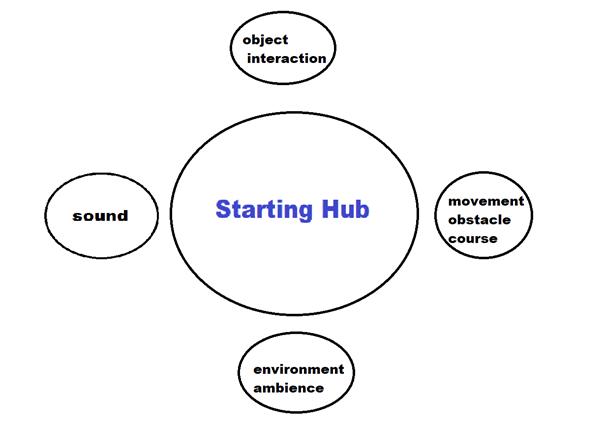
\includegraphics[width=12cm]{Chapters/Picture2.png}

\subsection{User Testing and Data Processing}
The testing was originally planned to be performed in person through on campus volunteers however due to the Covid-19 virus situation in the current year this might not be an option. 
This process might create unexpected difficulties as this means that we need to locate volunteers which have their own Virtual Reality systems to conduct the tests on.  

The tests will be done in a survey format following each of the tests, the users will have to answer questions such as their level of immersion during the test, which factors of the test aided to the immersion and which factors took away from the immersion factor. 

The results will be collected which will be gathered on a Microsoft Excel spreadsheet to analyse, compile, and chart the data. This data will be documented and used to form an idea of which factors are important to consider when attempting to create a virtual reality experience. 



 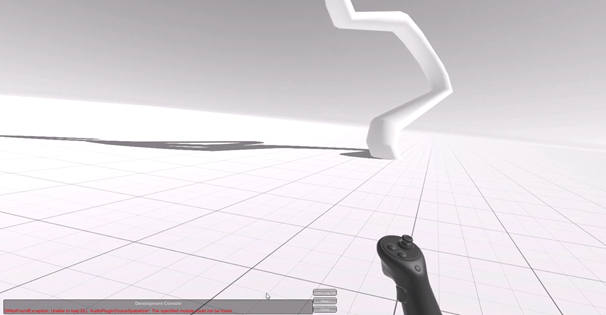
\includegraphics[width=15cm]{Chapters/Picture3.png}




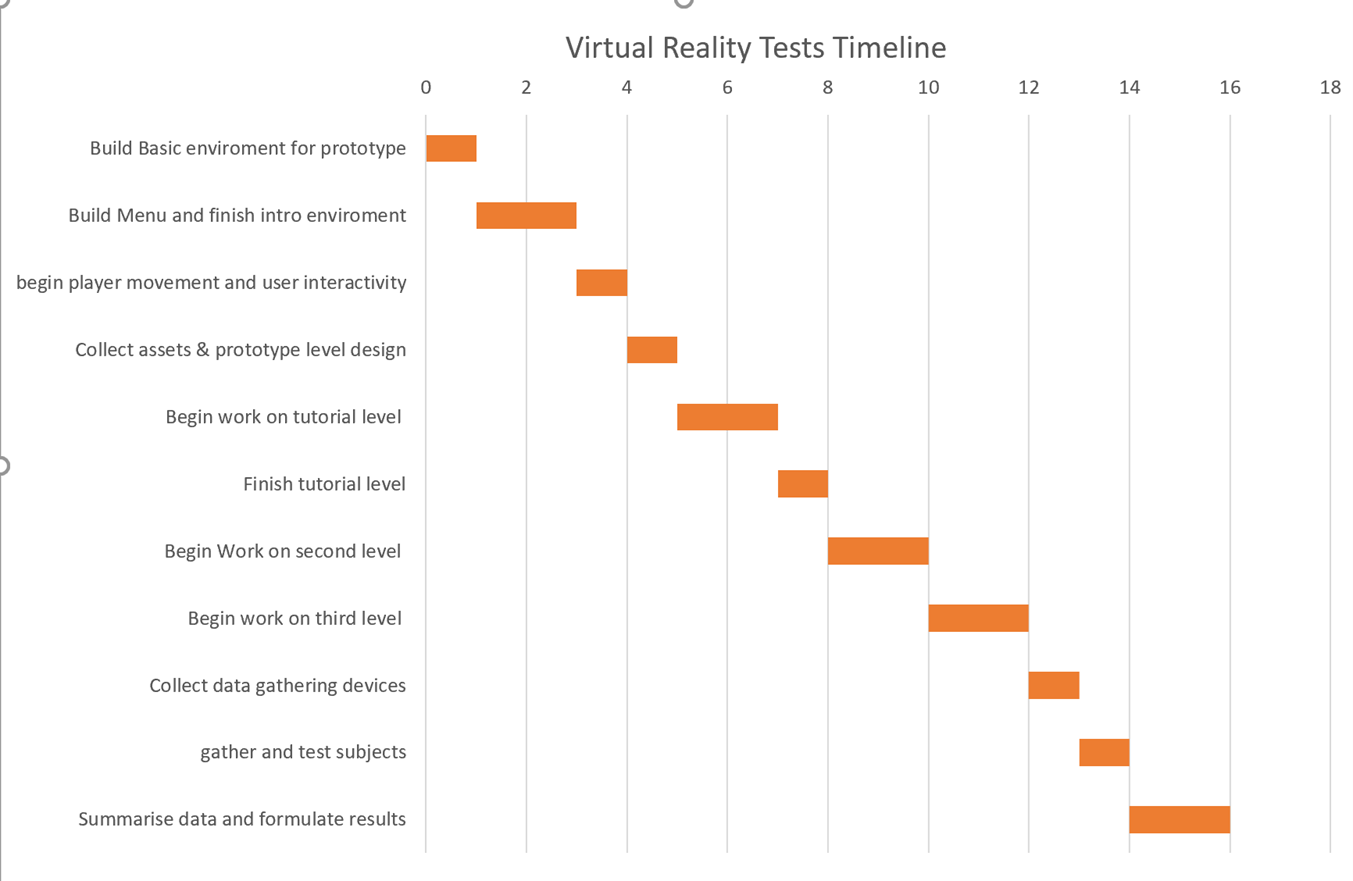
\includegraphics[width=15cm]{Chapters/Picture4.png}
